% !TEX root = ../report.tex
\chapter{Konzept}
\begin{Spacing}{\mylinespace}

\section{Datenfluss}
Der Datenfluss unseres Projektes soll hiermit noch einmal mit einer kurzen Skizze erläutert werden.
Als erstes wird ein Tiefenbild mit der Kinekt erfasst und an unsere Applikation übermittelt.
Die Applikation verarbeitet die erfassten Daten und bereitet diese für die GPU vor.
Anschließend arbeitet die GPU auf den erfassten Daten und erzeugt ein Bild welches auf dem Bildschirm bzw. Beamer erscheint.
\begin{figure}[h!]
	\centering
	\vspace*{20px}
	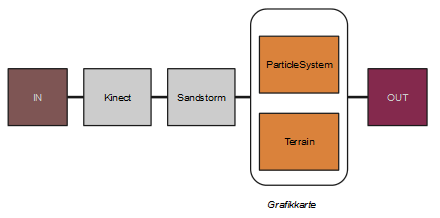
\includegraphics[width=250px]{graphics/flow.png}
	\caption{Datenfluss}
	\label{fig:dataFlow}
\end{figure}

\section{Modularisierung}
Um eine parallele Entwicklung und spätere Erweiterbarkeit sicherzustellen entschieden wir uns für eine modulbasierte Entwicklung.
Unser Projekt lässt sich in 3 Kategorien gliedern. Das ParticleSystem \textbf{(ParticleSystem)}, die Kinect Ansteuerung \textbf{(SandstormKinect)} und einen Controller \textbf{(Sandstorm)} der Events entgegen nimmt und diese verarbeitet oder ggf. weiterleitet.
Das XNA-Framework unterstützt einen modulbasierten Ansatz indem es jeder DrawableGameCompontent ihren eigenen Kontext zuweist.
Dies bedeutet das jede DrawableGameCompontent ein eigenes kleines Projekt darstellt und unabhängig von den anderen Projekten betrieben werden kann.
\begin{figure}[h!]
	\centering
	\vspace*{20px}
	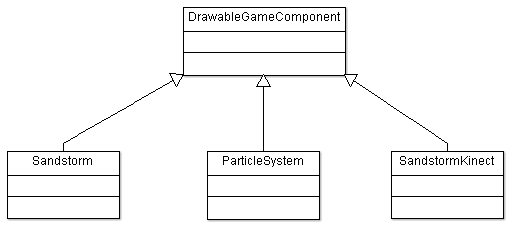
\includegraphics[width=320px]{graphics/DrawableGame.png}
	\caption{Kompontenten}
	\label{fig:singleColor}
\end{figure}

\section{Versionierung}
Um einen bestmöglichsten Konfort während der parallelen Entwicklung zu gewährleisten benötigt es neben der Synchronisierung auch eine Versionierung von Quellcode. Es gibt diverse Ansätze um dies sicherzustellen jedoch bieten Tools wie SVN, CVS, Perforce oder GIT sehr ähnliche Funktionlitäten. Wir entschieden uns aus Gewohnheit für ein GIT-Repository auf Github.com, dies lies sich innerhalb von Minuten einrichten und ist überall - sofern eine Internetverbindung besteht - erreichbar. Jeglicher Quellcode des Projekts lässt sich somit unter folgender Adresse abrufen: \url{https://github.com/tsturm/sandstorm}. Zusätzlich wird auf dem Perforce-Server des Fachbereichs Informatik die aktuelle Version vorgehalten.


\section{Properties}
Um unser System so dynamisch wie möglich zu gestalten entschlossen wir uns diverse Sammelcontainer für Systemparameter einzuführen - sogenannte Properties.
Diese Properties sind vergleichbar mit Konfigurationsdateien. Ändert man einen Wert innerhalb einer Properties so wird der neue Wert sofort vom restlichen System übernommen.
Dadurch das jegliche Parameter einer Kategorie (Physikengine,RenderEngine,Kinect..) mit solch einer Properties ausgestattet sind, ist es möglich für verschiedene Anwendungscenarien Default-Wert zu hinterlegen und diese bei Bedarf zu laden oder zu speichern.

\end{Spacing}
\newpage
\clearpage
%% End Of Doc